\chapter{Performance Evaluation and Analysis}
\label{sec:pa}
\label{sec:performance}


For the code generation, we instruct
the compiler via directives to unroll the
innermost loops of Algorithms~\ref{alg:algo:fw} and \ref{alg:algo:bw}, i.\,e.,
to perform an unrolling over the rows.
Here, an unrolling factor of eight or 16 showed the best
performance for all architectures.
%
We prohibit vectorization of these loops, which causes the
compiler to use scalar floating point addition/multiplication or FMA
instructions.
%
We observe that
%\mycomment{OR: Dies ist doch eine gewonnene Erkenntnis, oder? => We observe that}
with vectorization enabled for these loops the compiler
performs manual gather and scatter, which results in the same or even poorer
performance compared to the scalar unrolled versions.
This is required as AVX2 only includes a vector gather instruction.
%
Only for the 1-way column unrolling of the sparse triangular solve
%\mycomment{OR: alle ``sparse solve'' durch ``forward/backward substitution'' ersetzen}
with KNL the compiler
generated loop utilizing vector scatter/gather instructions is superior to
the scalar version, which is why we use this version for the combination of KNL
and 1-way column unrolling.
However, SKX also supports vector scatter/gather instructions, but did not
show any performance improvement.

\begin{figure}[t]%
\centering%
\captionsetup[subfigure]{justification=centering,farskip=0pt}
\subfloat[][

IVB]{%
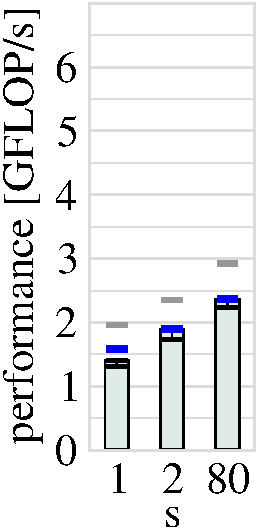
\includegraphics[height=2.9cm,clip=true]{images/perf/ps-n-20000/p-single-core-emmy-n-20000}
} %
\subfloat[HSW-D]{%
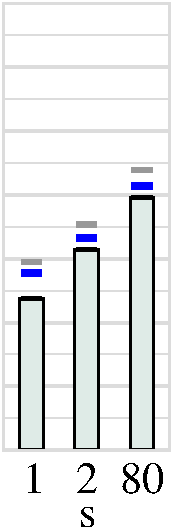
\includegraphics[height=2.9cm,clip=true]{images/perf/ps-n-20000/p-single-core-woody-hsw-n-20000}
} %
\subfloat[HSW-S]{%
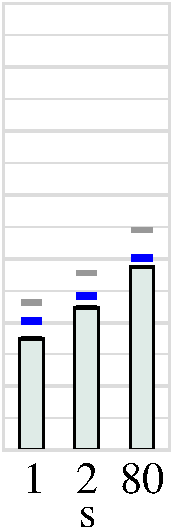
\includegraphics[height=2.9cm,clip=true]{images/perf/ps-n-20000/p-single-core-hasep1-n-20000}
} %
\subfloat[][

BDW]{%
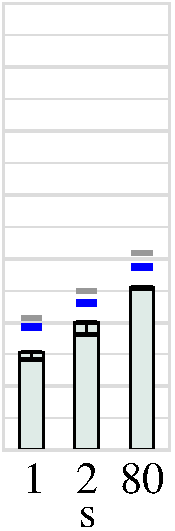
\includegraphics[height=2.9cm,clip=true]{images/perf/ps-n-20000/p-single-core-meggie-n-20000}
} %
\subfloat[][

SKX]{%
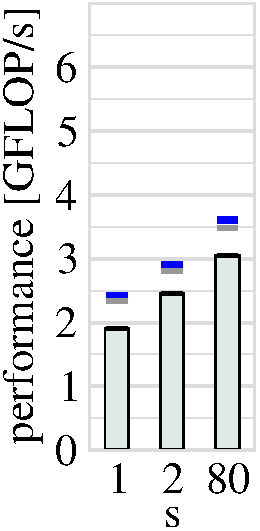
\includegraphics[height=2.9cm,clip=true]{images/perf/ps-n-20000/p-single-core-skylakesp2-n-20000}
} %
\subfloat[][

KNL]{%
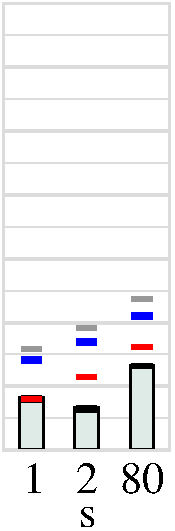
\includegraphics[height=2.9cm,clip=true]{images/perf/ps-n-20000/p-single-core-knightmare1-n-20000}
\label{fig:p:single-core:knl}
} %
\subfloat[ZEN-D]{%
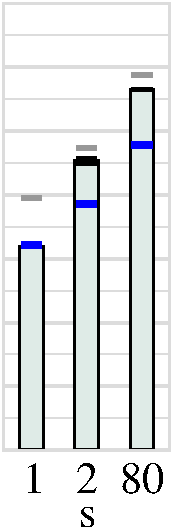
\includegraphics[height=2.9cm,clip=true]{images/perf/ps-n-20000/p-single-core-summitridge1-n-20000}
\label{fig:p:single-core:zen-d}
} %
\subfloat[ZEN-S]{%
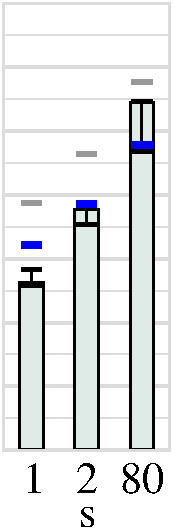
\includegraphics[height=2.9cm,clip=true]{images/perf/ps-n-20000/p-single-core-naples1-n-20000}
\label{fig:p:single-core:zen-s}
} %
  \caption{Performance of PARDISO's sparse triangular solve
    %with $1$-, $2$-, and $8$-way column unrolling 
    for the matrix \mymat{dense}. % with panel size $\panelsize = 1$, $2$,
    %and $80$, respectively.
    Blue and gray horizontal bars show predictions of the modified roofline model 
    with scalar and vectorized read bandwidth, respectively.
    }%
  \label{fig:p:single-core}%
\end{figure}

\begin{figure*}%
  \centering%
  
 \begin{tabular}{lcccccccc}
 %\begin{tabular}{>{\tiny \bfseries}lcccccccccc>{\tiny \bfseries}lccccccccccc}
 &
 \multicolumn{1}{c}{\tiny \bfseries IVB} & \multicolumn{1}{c}{\tiny \bfseries
HSW-D} & \multicolumn{1}{c}{\tiny \bfseries HSW-S} & \multicolumn{1}{c}{\tiny
\bfseries BDW} & \multicolumn{1}{c}{\tiny \bfseries SKX} &
\multicolumn{1}{c}{\tiny \bfseries KNL} & \multicolumn{1}{c}{\tiny \bfseries
ZEN-D} & \multicolumn{1}{c}{\tiny \bfseries ZEN-S} \\

% start matrix lapl1 (n-40-b-4)
 \raisebox{1.70cm}{\rotatebox[origin=c]{90}{lapl1}} &
  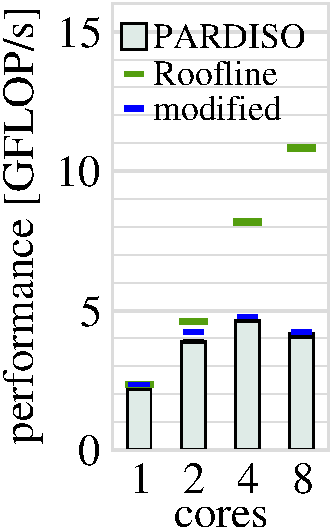
\includegraphics[height=3.0cm,clip=true]{images/perf/p-80/p-emmy-n-40-b-4}% 
  & 
  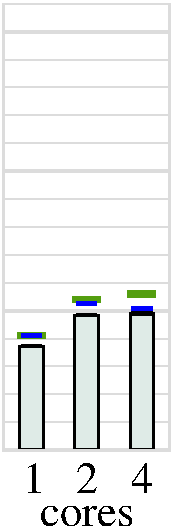
\includegraphics[height=3.0cm,clip=true]{images/perf/p-80/p-woody-hsw-n-40-b-4}% 
  & 
  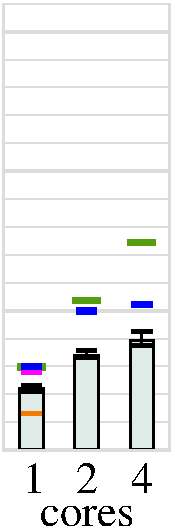
\includegraphics[height=3.0cm,clip=true]{images/perf/p-80/p-hasep1-n-40-b-4}% 
  & 
  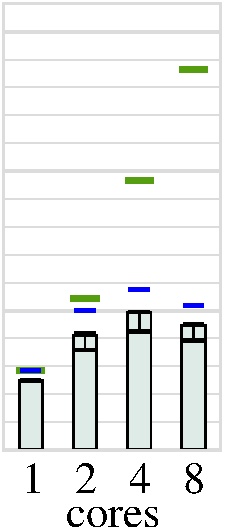
\includegraphics[height=3.0cm,clip=true]{images/perf/p-80/p-meggie-n-40-b-4}% 
  & 
  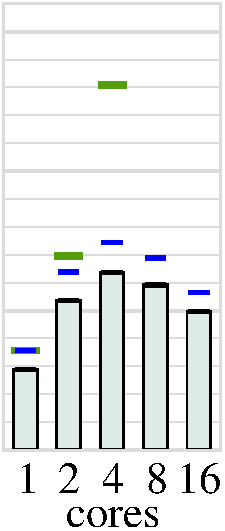
\includegraphics[height=3.0cm,clip=true]{images/perf/p-80/p-skylakesp2-n-40-b-4}% 
  & 
  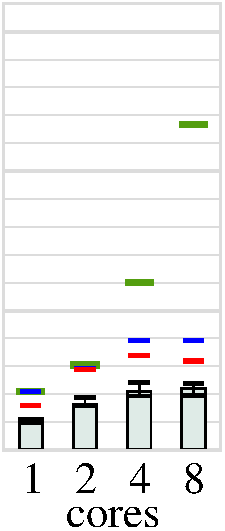
\includegraphics[height=3.0cm,clip=true]{images/perf/p-80/p-knightmare1-n-40-b-4}% 
  & 
  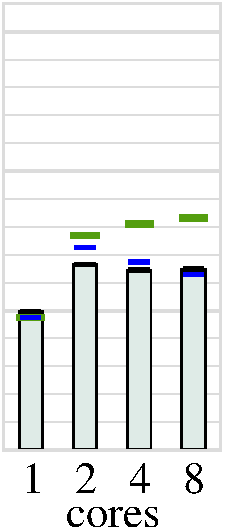
\includegraphics[height=3.0cm,clip=true]{images/perf/p-80/p-summitridge1-n-40-b-4}% 
  & 
  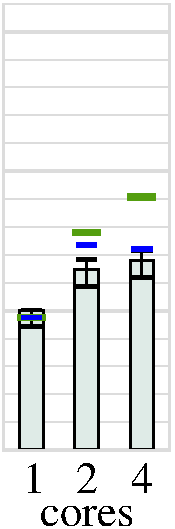
\includegraphics[height=3.0cm,clip=true]{images/perf/p-80/p-naples1-n-40-b-4}% 
%
\\
% end matrix n-40-b-4
% start matrix lapl2 (n-70-b-1)
 \raisebox{1.70cm}{\rotatebox[origin=c]{90}{lapl2}} &
  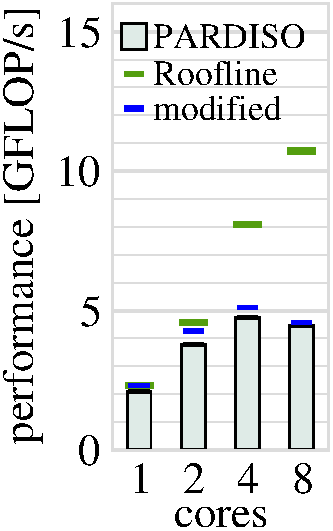
\includegraphics[height=3.0cm,clip=true]{images/perf/p-80/p-emmy-n-70-b-1}% 
  & 
  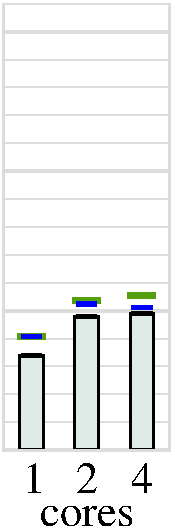
\includegraphics[height=3.0cm,clip=true]{images/perf/p-80/p-woody-hsw-n-70-b-1}% 
  & 
  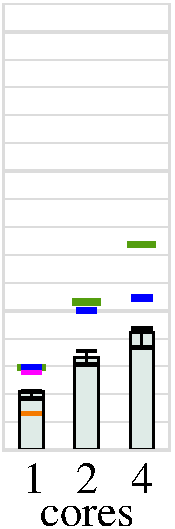
\includegraphics[height=3.0cm,clip=true]{images/perf/p-80/p-hasep1-n-70-b-1}% 
  & 
  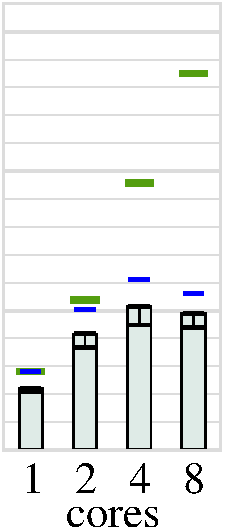
\includegraphics[height=3.0cm,clip=true]{images/perf/p-80/p-meggie-n-70-b-1}% 
  & 
  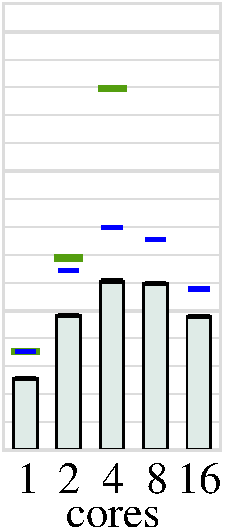
\includegraphics[height=3.0cm,clip=true]{images/perf/p-80/p-skylakesp2-n-70-b-1}% 
  & 
  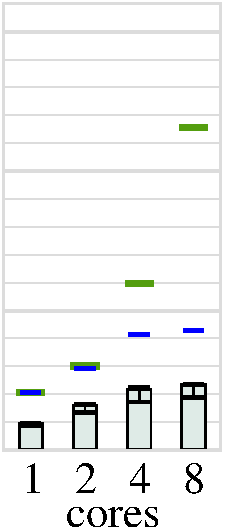
\includegraphics[height=3.0cm,clip=true]{images/perf/p-80/p-knightmare1-n-70-b-1}% 
  & 
  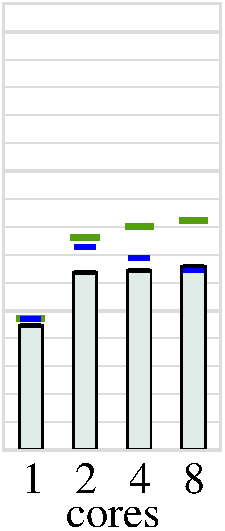
\includegraphics[height=3.0cm,clip=true]{images/perf/p-80/p-summitridge1-n-70-b-1}% 
  & 
  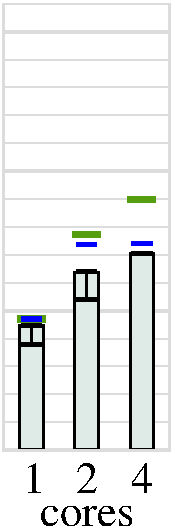
\includegraphics[height=3.0cm,clip=true]{images/perf/p-80/p-naples1-n-70-b-1}% 
\\
% end matrix n-70-b-1
% start matrix feti1 (mat_Kii_sd22_size750141_load2_newton1)
 \raisebox{1.70cm}{\rotatebox[origin=c]{90}{bddc1}} &
  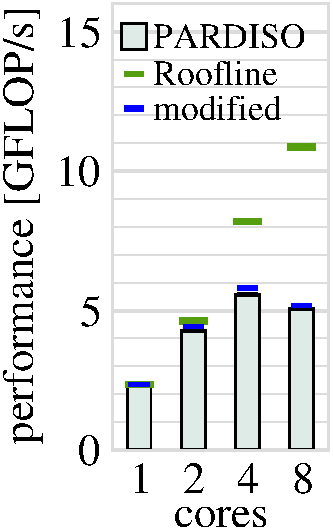
\includegraphics[height=3.0cm,clip=true]{images/perf/p-80/p-emmy-mat_Kii_sd22_size750141_load2_newton1}% 
  & 
  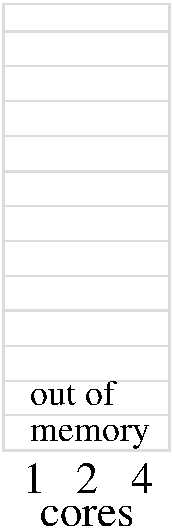
\includegraphics[height=3.0cm,clip=true]{images/perf/p-80/p-woody-hsw-mat_Kii_sd22_size750141_load2_newton1}% 
  & 
  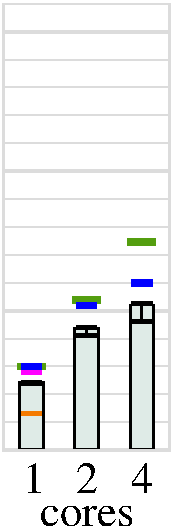
\includegraphics[height=3.0cm,clip=true]{images/perf/p-80/p-hasep1-mat_Kii_sd22_size750141_load2_newton1}% 
  & 
  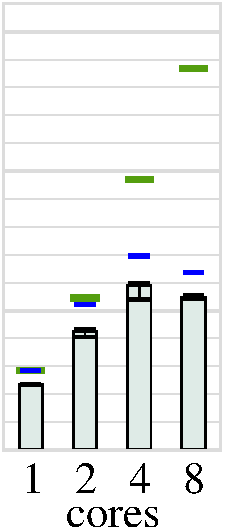
\includegraphics[height=3.0cm,clip=true]{images/perf/p-80/p-meggie-mat_Kii_sd22_size750141_load2_newton1}% 
  & 
  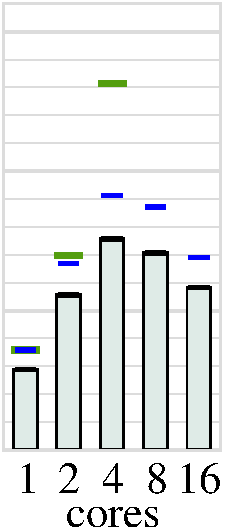
\includegraphics[height=3.0cm,clip=true]{images/perf/p-80/p-skylakesp2-mat_Kii_sd22_size750141_load2_newton1}% 
  & 
  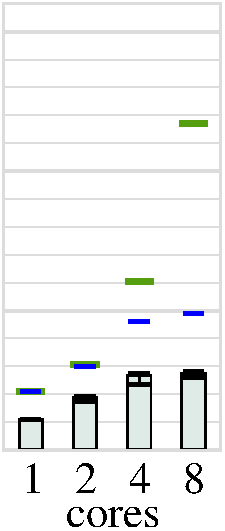
\includegraphics[height=3.0cm,clip=true]{images/perf/p-80/p-knightmare1-mat_Kii_sd22_size750141_load2_newton1}% 
  & 
  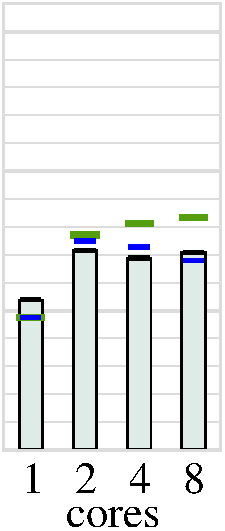
\includegraphics[height=3.0cm,clip=true]{images/perf/p-80/p-summitridge1-mat_Kii_sd22_size750141_load2_newton1}% 
  & 
  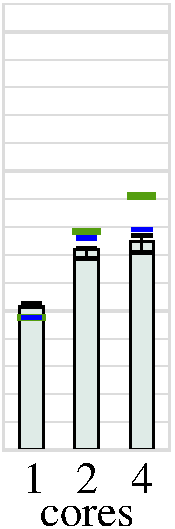
\includegraphics[height=3.0cm,clip=true]{images/perf/p-80/p-naples1-mat_Kii_sd22_size750141_load2_newton1}% 
\\



% &
% \multicolumn{1}{c}{\tiny \bfseries IVB} & \multicolumn{1}{c}{\tiny \bfseries
%HSW-D} & \multicolumn{1}{c}{\tiny \bfseries HSW-S} & \multicolumn{1}{c}{\tiny
%\bfseries BDW} & \multicolumn{1}{c}{\tiny \bfseries SKX} &
%\multicolumn{1}{c}{\tiny \bfseries KNL} & \multicolumn{1}{c}{\tiny \bfseries
%ZEN-D} & \multicolumn{1}{c}{\tiny \bfseries ZEN-S} \\

% start matrix lapl1 (n-40-b-4)
\raisebox{1.70cm}{\rotatebox[origin=c]{90}{omen1}} &
  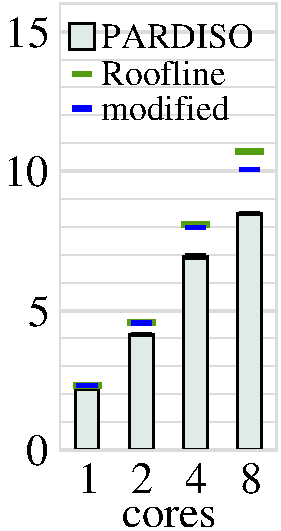
\includegraphics[height=3.0cm,clip=true]{images/perf/p-80/p-emmy-omen-rgf-tc2_5-lc160}% 
  & 
  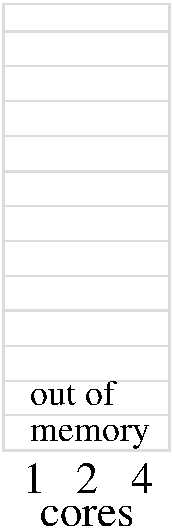
\includegraphics[height=3.0cm,clip=true]{images/perf/p-80/p-woody-hsw-omen-rgf-tc2_5-lc160}% 
  & 
  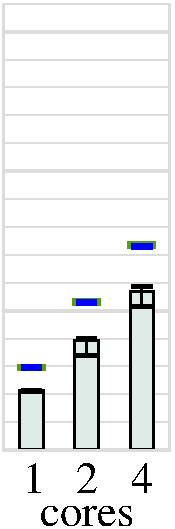
\includegraphics[height=3.0cm,clip=true]{images/perf/p-80/p-hasep1-omen-rgf-tc2_5-lc160}% 
  & 
  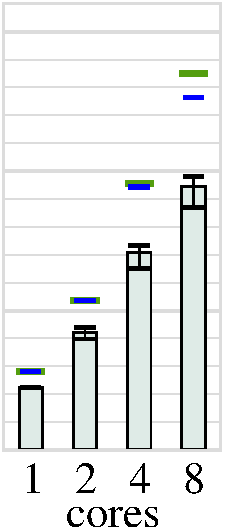
\includegraphics[height=3.0cm,clip=true]{images/perf/p-80/p-meggie-omen-rgf-tc2_5-lc160}% 
  & 
  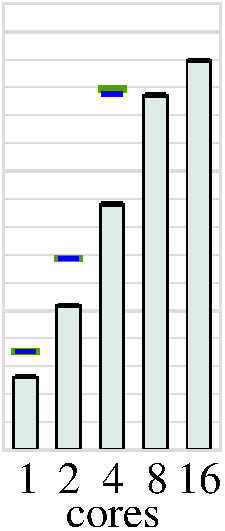
\includegraphics[height=3.0cm,clip=true]{images/perf/p-80/p-skylakesp2-omen-rgf-tc2_5-lc160}% 
  & 
  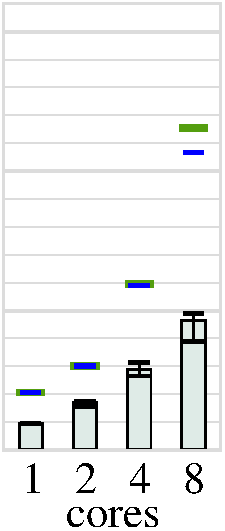
\includegraphics[height=3.0cm,clip=true]{images/perf/p-80/p-knightmare1-omen-rgf-tc2_5-lc160}% 
  & 
  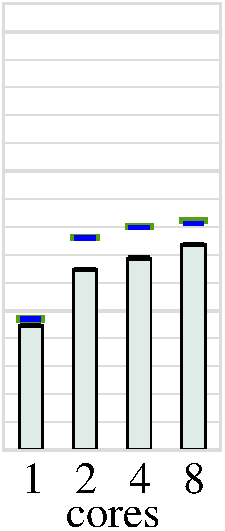
\includegraphics[height=3.0cm,clip=true]{images/perf/p-80/p-summitridge1-omen-rgf-tc2_5-lc160}% 
  & 
  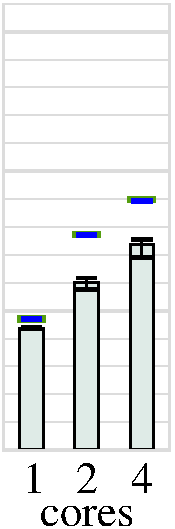
\includegraphics[height=3.0cm,clip=true]{images/perf/p-80/p-naples1-omen-rgf-tc2_5-lc160}% 
\\
% end matrix n-40-b-4
% start matrix lapl2 (n-70-b-1)
\raisebox{1.70cm}{\rotatebox[origin=c]{90}{omen2}} &
  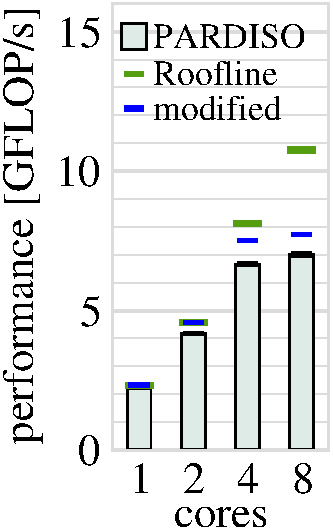
\includegraphics[height=3.0cm,clip=true]{images/perf/p-80/p-emmy-omen-rgf-tc3_5}% 
  & 
  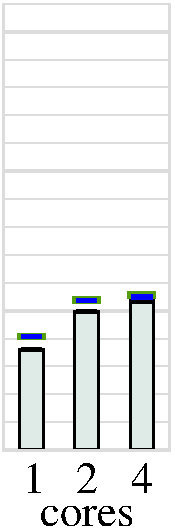
\includegraphics[height=3.0cm,clip=true]{images/perf/p-80/p-woody-hsw-omen-rgf-tc3_5}% 
  & 
  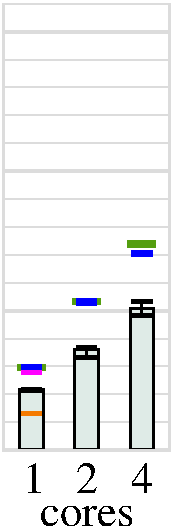
\includegraphics[height=3.0cm,clip=true]{images/perf/p-80/p-hasep1-omen-rgf-tc3_5}% 
  & 
  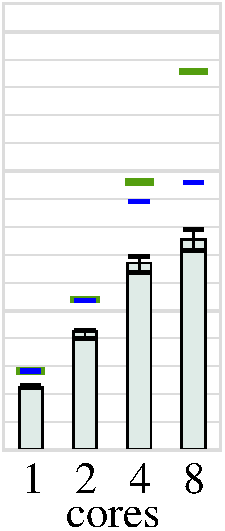
\includegraphics[height=3.0cm,clip=true]{images/perf/p-80/p-meggie-omen-rgf-tc3_5}% 
  & 
  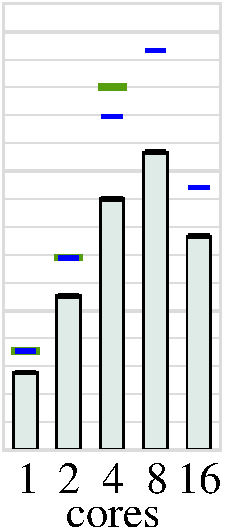
\includegraphics[height=3.0cm,clip=true]{images/perf/p-80/p-skylakesp2-omen-rgf-tc3_5}% 
  & 
  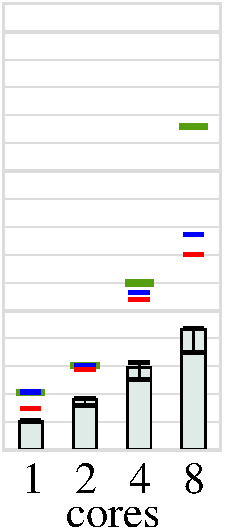
\includegraphics[height=3.0cm,clip=true]{images/perf/p-80/p-knightmare1-omen-rgf-tc3_5}% 
  & 
  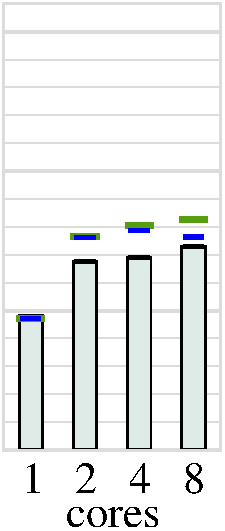
\includegraphics[height=3.0cm,clip=true]{images/perf/p-80/p-summitridge1-omen-rgf-tc3_5}% 
  & 
  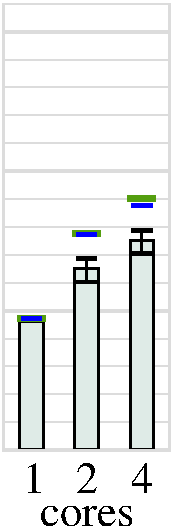
\includegraphics[height=3.0cm,clip=true]{images/perf/p-80/p-naples1-omen-rgf-tc3_5}% 
\\
% end matrix n-70-b-1
% start matrix feti1 (mat_Kii_sd22_size750141_load2_newton1)
\raisebox{1.70cm}{\rotatebox[origin=c]{90}{omen3}} &
  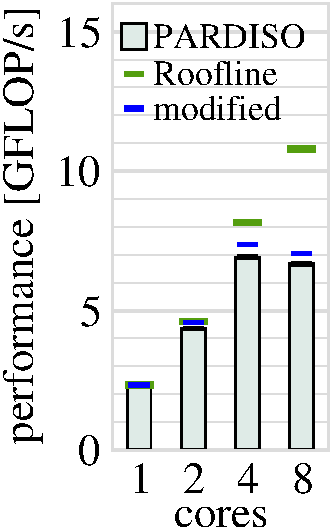
\includegraphics[height=3.0cm,clip=true]{images/perf/p-80/p-emmy-omen-rgf-tc4_5}% 
  & 
  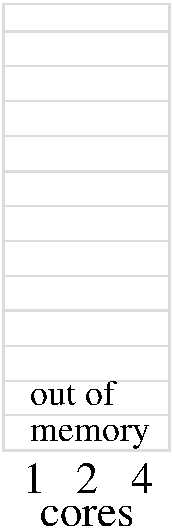
\includegraphics[height=3.0cm,clip=true]{images/perf/p-80/p-woody-hsw-omen-rgf-tc4_5}% 
  & 
  \includegraphics[height=3.0cm,clip=true]{images/perf/p-80/p-hasep1-omen-rgf-tc4_5}% 
  & 
  \includegraphics[height=3.0cm,clip=true]{images/perf/p-80/p-meggie-omen-rgf-tc4_5}% 
  & 
  \includegraphics[height=3.0cm,clip=true]{images/perf/p-80/p-skylakesp2-omen-rgf-tc4_5}% 
  & 
  \includegraphics[height=3.0cm,clip=true]{images/perf/p-80/p-knightmare1-omen-rgf-tc4_5}% 
  & 
  \includegraphics[height=3.0cm,clip=true]{images/perf/p-80/p-summitridge1-omen-rgf-tc4_5}% 
  & 
  \includegraphics[height=3.0cm,clip=true]{images/perf/p-80/p-naples1-omen-rgf-tc4_5}% 
\\


% end matrix omen-rgf-tc4.5
% &
%&\tiny \makecell{$e = $ \\ $[-1, 18 ]$}&\tiny \makecell{$e = $ \\ $[0, 19 ]$}&\tiny \makecell{$e = $ \\ $[15, 51 ]$}&\tiny \makecell{$e
%= $ \\ $[14, 33 ]$}&\tiny \makecell{$e = $ \\ $[13, 62 ]$}&\tiny \makecell{$e = $ \\ $[59, 129 ]$}&\tiny \makecell{$e = $ \\ $[-11, 17
%]$}&\tiny \makecell{$e = $ \\ $[-7, 28 ]$}
%
%&&
%
% &
%&\tiny \makecell{$e = $ \\ $[-1, 18 ]$}&\tiny \makecell{$e = $ \\ $[0, 19 ]$}&\tiny \makecell{$e = $ \\ $[15, 51 ]$}&\tiny \makecell{$e
%= $ \\ $[14, 33 ]$}&\tiny \makecell{$e = $ \\ $[13, 62 ]$}&\tiny \makecell{$e = $ \\ $[59, 129 ]$}&\tiny \makecell{$e = $ \\ $[-11, 17
%]$}&\tiny \makecell{$e = $ \\ $[-7, 28 ]$}
\end{tabular}
%
%
  %
  \caption{Performance of sparse triangular solve with benchmark matrices of
panel size $s=80$ on one NUMA LD for each hardware system.
  Green and blue bars show predictions of the original and modified roofline
model, respectively.
  HSW-S and ZEN-S have 14 and 24 cores in total and using all cores could
achieve, with correct NUMA placement, a higher performance, respectively. 
  Bottom row shows the model error $e$ for the corresponding system in
percentage.}%
  \label{fig:p:pardiso}
\end{figure*}

For the single core measurements we use the matrix \mymat{dense}.
We create three variants of it, where the maximum panel size $\panelsize$ is
limited to $1$, $2$, and $80$ columns.
This enables isolated measurement of the $1$-, $2$-, and $8$-way
unrolled loops.
Furthermore, the matrix \mymat{dense} exhibits the most homogeneous access pattern
as memory is only accessed in long contiguous streams and relates best to our
read-only benchmark (section~\ref{sec:tb:membw}) used as input for the modified
roofline model (section~\ref{sec:mrm}, \eqref{eq:rm:mod}).
%
Figure~\ref{fig:p:single-core} shows the measured performance for all systems in
our testbed for sparse triangular solve.
The blue bars indicate the performance limit from the modified roofline model.
%
In general larger panels deliver a higher performance.
This is expected as the code balance decreases with increasing panel sizes.
For panel sizes $s=1$ and $s=2$ with matrix \mymat{dense}, the worst case code balance
of $B_c=6$\,B/F and $B_c=5$\,B/F is reached, respectively. 
With a panel size $s=80$ the code balance for the $8$-way unrolled loop
becomes nearly $B_c=4$\,B/F.
  
The modified roofline model predictions for the Intel based systems (except for
KNL) deviate up to $25$\,\% from the measurements, but achieve a higher
performance with larger panels.
%
For KNL the model error is in the range of $55$\,\% to $160$\,\% over all panel
sizes which suggests some error in the model assumptions.
On KNL a STREAM-like (scalar) copy and read benchmark achieves an L2 bandwidth of
around $7.8$\,GB/s and $8.5$\,GB/s with one core,
respectively.
From Figure~\ref{fig:ecm:data}, we see that between the L1 and L2 caches (depending on
the matrix) we might have a higher code
balance compared to the one we assume between memory and L2.
As the measured L2 bandwidth is nearly equal to the memory read-only bandwidth
the former data path becomes the new bottleneck.
However, determining a priori the code balance between the L1 and L2 caches for a matrix
is analytically nontrivial which is why we derive the metric from the measured data
traffic between the caches.
The adjusted model based on these new inputs is shown in
Figure~\ref{fig:p:single-core:knl} as red bars and reduces the model error
significantly.
%
The poor performance with panel size $s = 2$, however, is unclear and deserves
further investigation. 
%
%
% The measured data traffic between memory and L2 is only about $5$\,\% higher
% than our model assumption for $s=1$ and $s=2$.
% With $s=80$ we measure a $25$\,\% increased amount of data.
% Despite the latter deviation is pretty large the increased memory traffic cannot
% (alone) account for the performance discrepancy on KNL.
% Currently we are still investigating this issue.
% \todo{multi stream?}
%
The roofline model for the AMD-based ZEN systems underestimates the
performance by up to $20$\,\%.
It seems that sparse solve in the cases of ZEN-D and $s=2, 80$ and ZEN-S and $s=80$
achieves the bandwidth obtained with the vectorized read benchmark as the bars
in Figures~\ref{fig:p:single-core:zen-d} and~\ref{fig:p:single-core:zen-s} match
the gray lines, which represent the modified roofline model based on the
vectorized read-only bandwidth.
Measuring the actual clock frequency shows that ZEN-D and ZEN-S run with
$3.8$\,GHz and $3.2$\,GHz during sparse solve, respectively.
However, they also achieve this frequency during read-only bandwidth
measurements.
Until now its unclear why both systems reach a higher bandwidth with sparse
solve compared to the scalar read-only benchmark.
% \todo{multi stream not the answer}
% As we are currently unable to measure the memory traffic on this architecture
% we cannot compare it to our model assumptions we have to postpone further
% investigations regarding this issue.
% \todo{only scalar FMA used}
%
%1 For the SX machine the modified Roofline model predictions exceed the graphs
%1 y-axis and are therefore not shown.
%1 As expected due to the high single core bandwidth the SX ACE outperforms all
%1 other machines.
% As the compiler already utilizes gather and scatter instructions and places
% vector $r$ in the ADB (assignable data buffer, a $1$\,MiB large vector cache) in
% both code versions, we did not explicitly include any other optimizations.

%%%%%%%%%%%%%%%%%%%%%%%%%%%%%%%%%%%%%%%%%%%%%%%%%%%%%%%%%%%%%%




Performance results for all matrices are shown in Figure~\ref{fig:p:pardiso}.
For HSW-D (second column) the main memory was not large enough for benchmarks
with the \mymat{bddc}, \mymat{omen2}, and \mymat{omen3} matrices, which is
indicated as ``out of memory'' in the figures.
%
%
Currently we only can ensure correct NUMA placement for one locality domain; this is why
we limit the scope of the analysis to one NUMA LD only. 
Hence, for HSW-S and ZEN-S fewer cores than the processor houses are used.
Please keep in mind that for HSW-S, seven of 14 cores and for ZEN-S only six of
24 cores are used and with correct NUMA placement and usage of more cores a
higher performance could be achieved.

%\begin{SCfigure}[2][t]%
\begin{figure}[t]%
  \centering%
  \includegraphics[width=0.5\textwidth,clip=true]{images/matrices-serial-fraction}%
  \caption{Fraction of nonzeros in the separator, which must be processed
   serially, depending on the number of cores for test matrices.  }%
  \label{fig:p:serial-fraciton}%
\end{figure}
%\end{SCfigure}

As already pointed out, the number of independent parallel parts produced by the
factorization is always a power of two.
For nonpower of two thread counts this results in load imbalance and decreases
performance, which is why we omit them in the graphs.
%
Furthermore, the current implementation of the factorization increases the size
of the separator in the factor $L$ with increasing number of threads as already
observed in scaling studies for sparse solve in~\cite{klawonn-2015}.
%
Figure~\ref{fig:p:serial-fraciton} shows the fraction of nonzeros in $L$ which are
part of the separator, i.\,e.,\ the part which must be executed serially.
Except for \mymat{omen1} this prohibits the efficient usage of larger core
counts and the test matrices reach their highest performance already with four
or eight cores.
%
This is also the reason why we cannot efficiently utilize KNL's high bandwidth
memory.
Despite its bandwidth scales (nearly) linearly with the number of cores, its
single core bandwidth is not significantly different from the one delivered from
main memory.
Only with higher core counts can the full HBM bandwidth be obtained.
However, with $16$, $32$, and $64$ threads the serial fraction of the resulting
factor from the matrices is already too high and performance nearly drops to
the single core performance level.
Hence, we excluded HBM measurements from the plots as it gives no further
insight.
%
With SKX hosting $20$ cores in one NUMA LD the impact of the separator becomes
visible (fifth column of Figure~\ref{fig:p:pardiso}).
The separator of \mymat{lapl1}, \mymat{lapl2}, and \mymat{bddc}\/ strongly increases 
over the number of cores and limits the scaling of the performance early.
The maximum performance here is already reached with four cores.
The increase of the serial fraction for \mymat{omen2} and \mymat{omen3} is not
that pronounced.
Here, the performance peak is reached with eight cores.
Only with \mymat{omen1}, where the separator stays small, performance increases
up to 16~cores.
All other architectures follow this pattern up to the number of cores used.

Figure~\ref{fig:p:pardiso} also shows the performance limits for the original
\eqref{eq:rm:simple} and the modified roofline model \eqref{eq:rm:mod}
as green and blue bars, respectively.
As the traditional model misses the serial fraction of the execution it scales
with the achievable bandwidth of the number of cores used.
This is increasingly pronounced, the larger the serial fraction becomes. 
%The gap between the models depends on two factors.
%Firstly the amount of the serial fraction of the matrix and secondly the ratio
%between the achievable memory bandwidth of the used cores compared to the single
%core bandwidth.
%
Systems saturating with one core nearly the total memory bandwidth exhibit
only a marginal gap, like HSW-D (second column in Figure~\ref{fig:p:pardiso}) or
slightly more pronounced ZEN-D (seventh column in Figure~\ref{fig:p:pardiso}).

In general the modified roofline model captures the behavior of the measured
performance over all systems and matrices as Figure~\ref{fig:p:pardiso} shows.
%
%
IVB and HSW-D, ZEN-D, and ZEN-S exhibit a model error of around $20$\,\% shown
in the bottom row of Figure~\ref{fig:p:pardiso}. 
For HSW-S, BDW, and SKX the model deviates up to $60$\,\% from the measurements.
%
% Especially the predictions for the \mymat{omen} matrices are around $10$\,\%
% worse than for the other matrices.
%
As measured data traffic is in the expected bounds a deeper analysis of the
architectures and algorithm is required.
One option for future investigations is the ECM performance
model (\cite{hager-2012-ecm}), which not only accounts for all transfers inside
the memory hierarchy but also performs an in-depth analysis of the execution in
the core.
%
%
For KNL the bottleneck with multiple cores becomes more complex than with a
single core.
The L2 bandwidth scales linearly with each core, whereas the memory bandwidth
scales only with pairs of cores, i.\,e.,\ per tile, and saturates at a certain
point.
Depending on the matrix and the size of its separator, L2 or memory bandwidth can
now be the bottleneck.
%
In order to keep the model simple, for KNL, we show
as red bars in Figure~\ref{fig:p:pardiso},
in addition
to the modified
roofline model, 
an adjusted version; cf.\ the single core measurements.
Here, we consider \mymat{lapl1} and \mymat{omen2}.
Note that all measurements might suffer from the poor performance of $2$-way
column unrolling.
%
% limited by shows the same behavior as with one core and matrix \mymat{dense}.
% Its performance stays far behind the predictions.
% 
HSW-D and ZEN-D can nearly saturate the memory bandwidth with one core and gain
nearly no benefit from using more than two cores.

% The gray lines in Fig.~\ref{fig:p:pardiso} show the modified Roofline model
% based on the vectorized read-only bandwidth. \todo{vectorization} 
% \todo{potential of vectorization}